\begin{table*}[h]
    \centering
    \resizebox{\textwidth}{!}{
        \begin{tabular}{c|c|c|c|c|c|c|c|c|c|c|c|c}
        batch size & audio length & sample rate & projector dim. & temperature & $p_{\mathrm{invert}}$ & $p_{\mathrm{noise}}$ & $p_{\mathrm{gain}}$ & $p_{\mathrm{filter}}$ & ROC-AUC$^{(\mathrm{MLP})}$ & PR-AUC$^{(\mathrm{MLP})}$ \\ \hline
        48 & 59049 & 22050 & 128 & 0.1 & 0.8 & 0.5 & 0.1 & 0.4 & \textbf{87.56} & 32.25 \\
        48 & 59049 & 22050 & 128 & 0.5 & 0.8 & 0.5 & 0.1 & 0.4 & 87.55 & 32.66 \\
        192	& 20736 & 8000 & 128 & 0.5 & 0.8 & 0.5 & 0.1 & 0.4 & 87.52 & 32.43 \\
        48	& 20736 & 8000 & 128 & 0.5 & 0.8 & 0.5 & 0.1 & 0.4 & 87.49 & 32.38 \\
        48 & 59049 & 22050 & 256 & 0.5 & 0.8 & 0.5 & 0.1 & 0.4 & 87.43 & 32.58 \\
        48 & 59049 & 22050 & 64	& 0.5 & 0.8 & 0.5 & 0.1 & 0.4 & 87.43 & 32.49 \\
        128 & 31104 & 12000	& 128 & 0.5 & 0.8 & 0.5 & 0.1	& 0.4 & 87.41 & \textbf{32.73} \\
        48 & 31104 & 12000 & 128 & 0.5 & 0.8 & 0.5 & 0.1 & 0.4 & 87.37 & 32.69 \\
        48 & 59049 & 22050 & 128 & 0.25 & 0.8 & 0.5 & 0.1 & 0.4 & 87.36 & 32.42 \\
        48 & 59049 & 22050 & 128 & 0.5 & 0.8 & 0.5 & 0.1 & 0.4 & 87.00 & 31.93 \\
        48 & 59049 & 22050 & 128 & 0.5 & 0.8 & 0.5 & 0.1 & 0 & 85.99 & 30.26 \\
        48 & 59049 & 22050 & 128 & 0.5 & 0.8 & 0 & 0 & 0 & 85.79 & 30.55 \\
        48 & 59049 & 22050 & 128 & 0.5 & 0.8 & 0.5 & 0 & 0 & 85.67 & 30.03 \\
        48	& 59049	& 22050	& 128 & 0.5	& 0 & 0 & 0 & 0	& 85.54 & 29.84 \\
        \end{tabular}
    }
    \caption{Ablation study of CLMR under different parameters, sampling rate and data augmentations. The ROC-AUC and PR-AUC scores are obtained with a logistic regression classifier with one hidden layer, and is trained only on the representations from a pre-trained, frozen CLMR network.}
    \label{tab:1}
\end{table*}


\begin{figure*}[h]
    \centering
    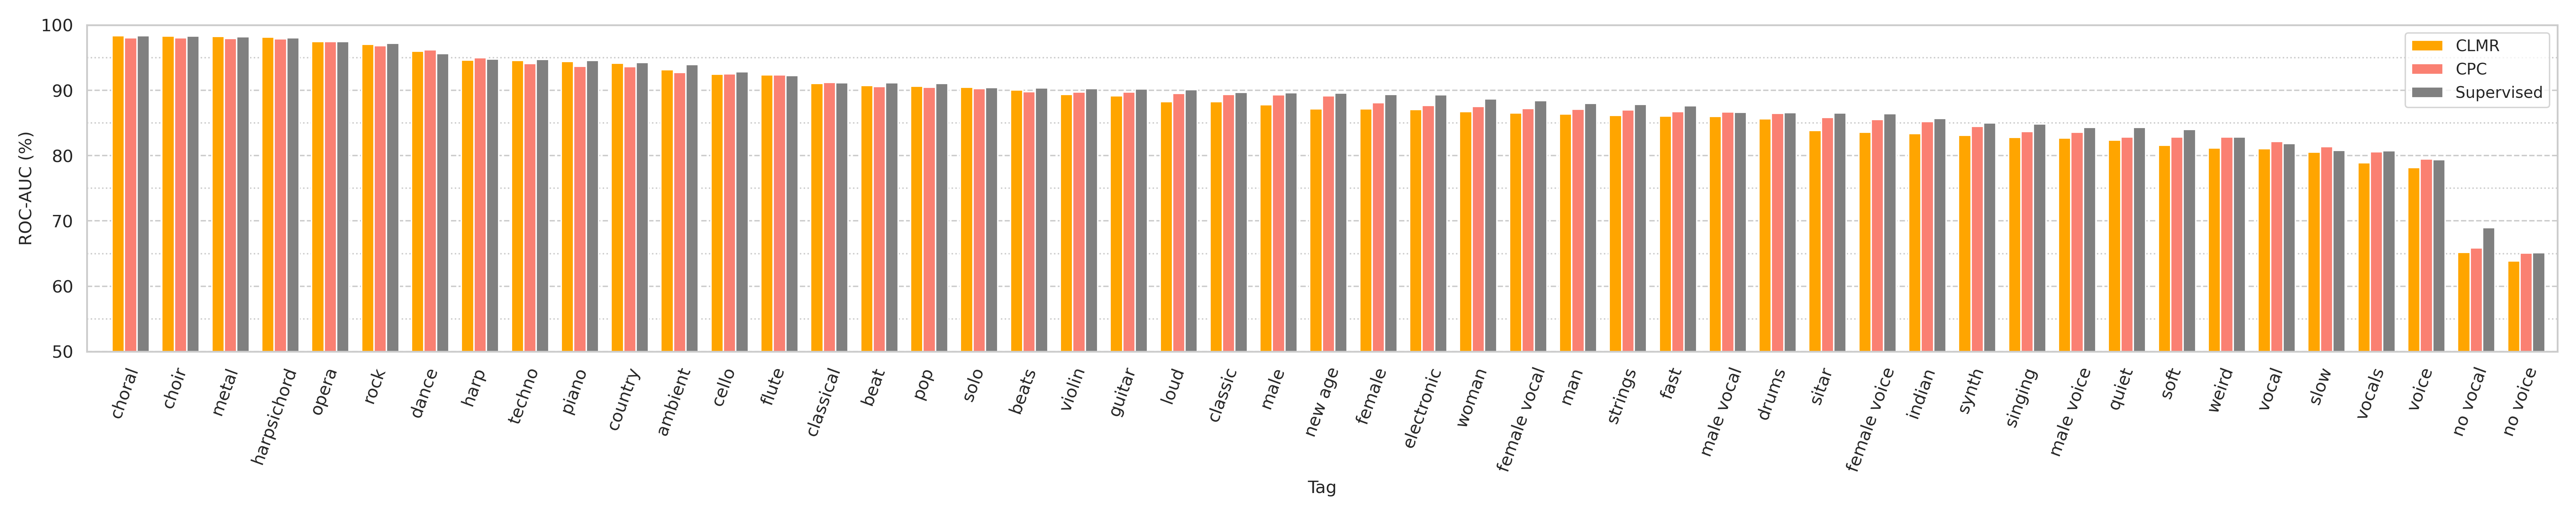
\includegraphics[width=\textwidth]{figs/tag_retrieval.png}
    \caption{Tag-wise ROC-AUC scores for the top-50 tags in the MagnaTagATune dataset, reported for linear, logistic regression classifiers trained on representations of self-supervised models CLMR and CPC, and compared to a fully supervised, end-to-end SampleCNN model.}
    \label{fig:tag_scores}
\end{figure*}



\begin{figure*}[h]
    \centering
    \subcaptionbox{CLMR$^{(1)}_{\mathrm{MTAT}}$\label{fig:1a}}{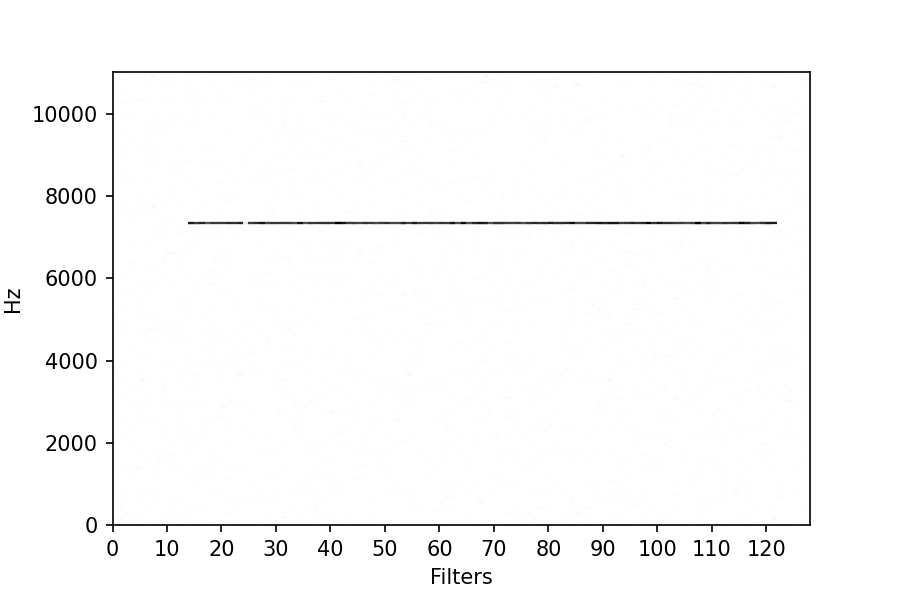
\includegraphics[width=.16\textwidth]{figs/magnatagatune/clmr_spectrum/epoch1490_layer0.png}}\hfill
    \subcaptionbox{CLMR$^{(4)}_{\mathrm{MTAT}}$\label{fig:1a}}{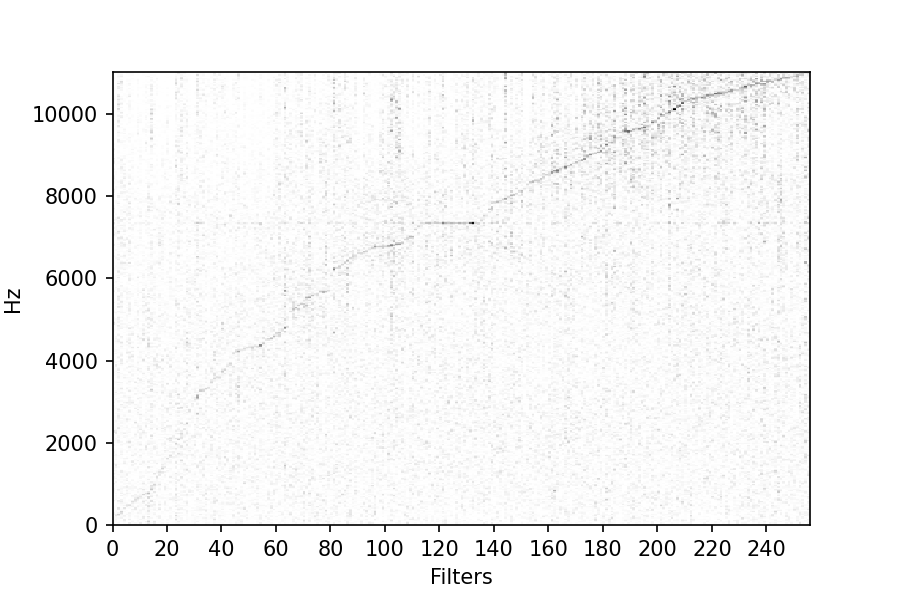
\includegraphics[width=.16\textwidth]{figs/magnatagatune/clmr_spectrum/epoch1490_layer3.png}}\hfill
    \subcaptionbox{CLMR$^{(6)}_{\mathrm{MTAT}}$\label{fig:1a}}{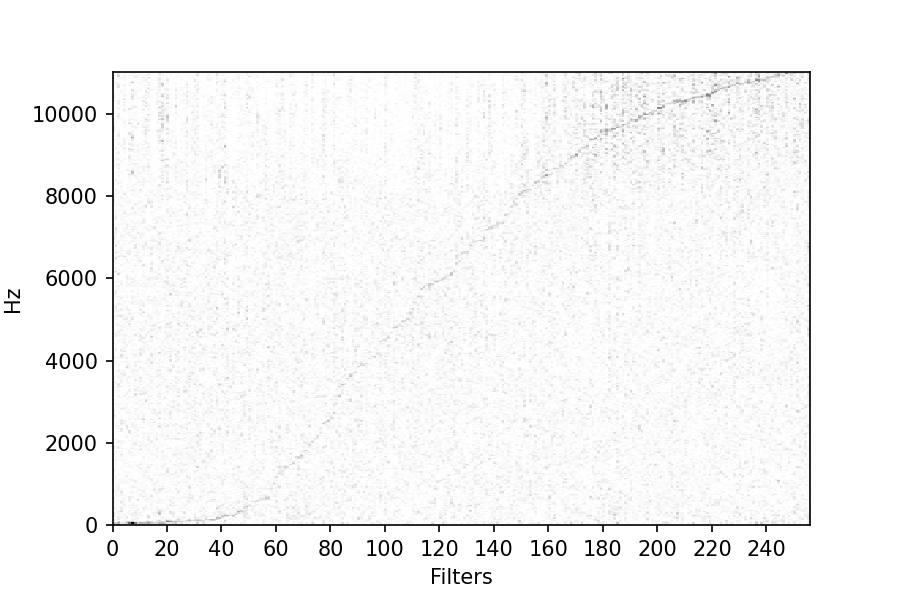
\includegraphics[width=.16\textwidth]{figs/magnatagatune/clmr_spectrum/epoch1490_layer5.png}}\hfill
    \subcaptionbox{CPC$^{(1)}_{\mathrm{MTAT}}$\label{fig:1a}}{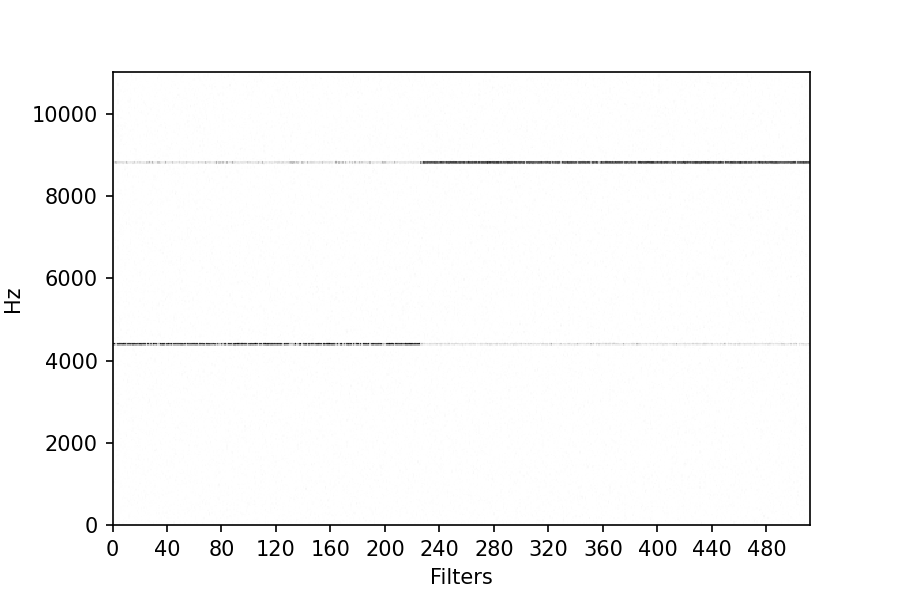
\includegraphics[width=.16\textwidth]{figs/magnatagatune/cpc_spectrum/epoch670_layer0.png}}\hfill
    \subcaptionbox{CPC$^{(4)}_{\mathrm{MTAT}}$\label{fig:1a}}{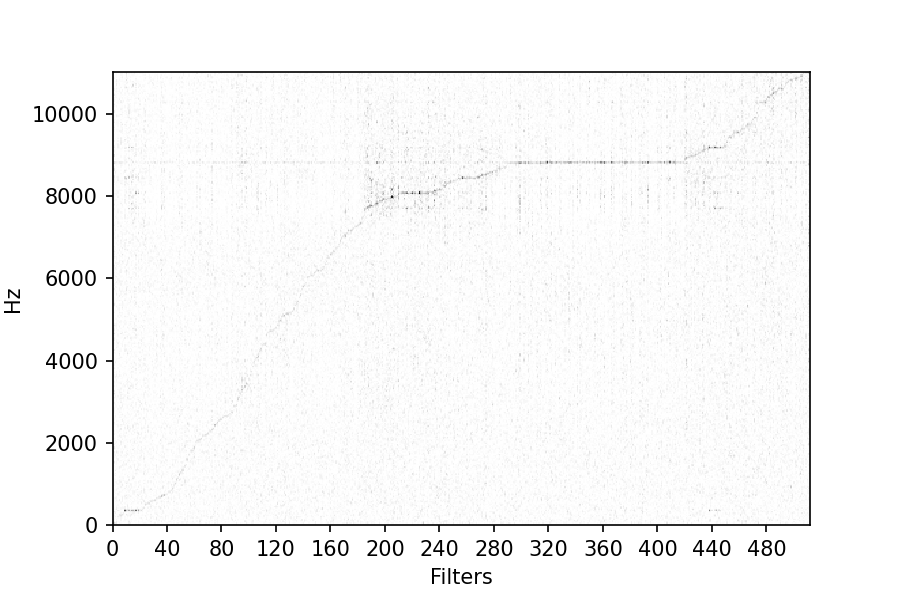
\includegraphics[width=.16\textwidth]{figs/magnatagatune/cpc_spectrum/epoch670_layer3.png}}\hfill
    \subcaptionbox{CPC$^{(6)}_{\mathrm{MTAT}}$\label{fig:1a}}{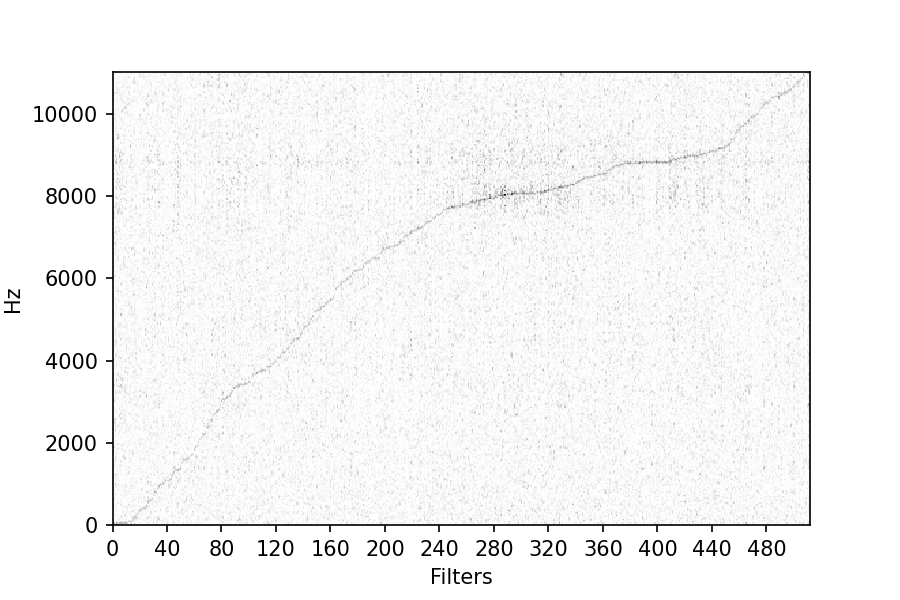
\includegraphics[width=.16\textwidth]{figs/magnatagatune/cpc_spectrum/epoch670_layer5.png}}

    \subcaptionbox{CLMR$^{(1)}_{\mathrm{Billboard}}$\label{fig:1a}}{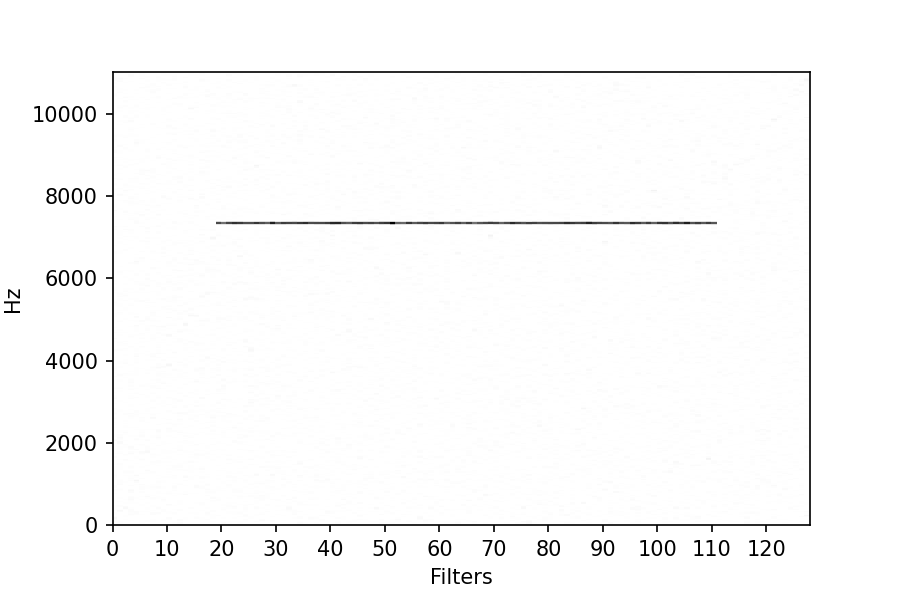
\includegraphics[width=.16\textwidth]{figs/billboard/clmr_spectrum/epoch1490_layer0.png}}\hfill
    \subcaptionbox{CLMR$^{(4)}_{\mathrm{Billboard}}$\label{fig:1a}}{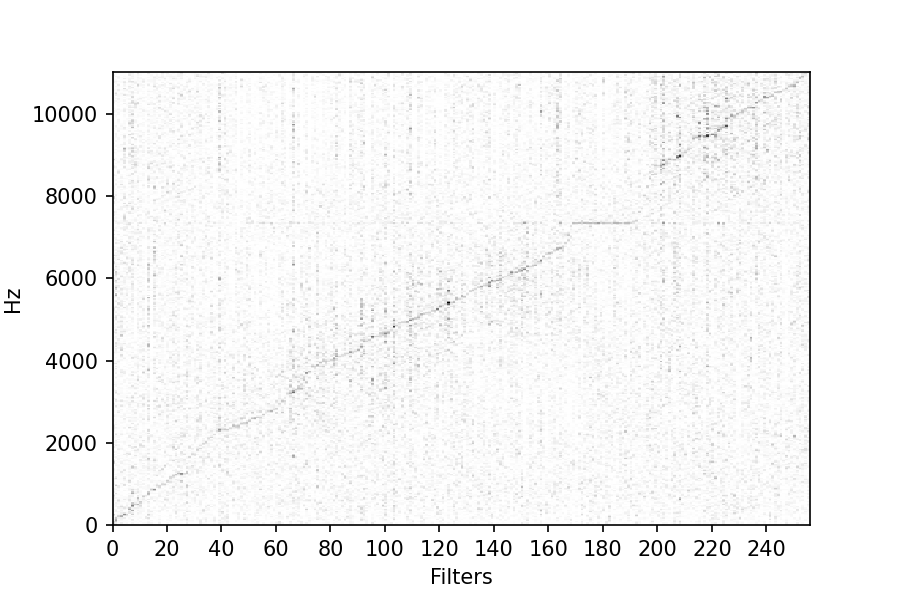
\includegraphics[width=.16\textwidth]{figs/billboard/clmr_spectrum/epoch1490_layer3.png}}\hfill
    \subcaptionbox{CLMR$^{(6)}_{\mathrm{Billboard}}$\label{fig:1a}}{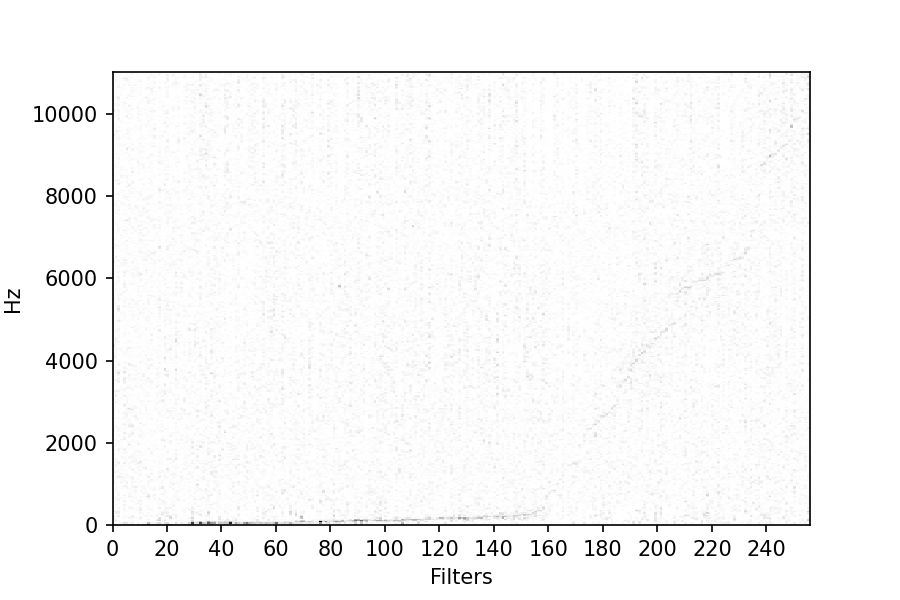
\includegraphics[width=.16\textwidth]{figs/billboard/clmr_spectrum/epoch1490_layer5.png}}\hfill
    \subcaptionbox{CPC$^{(1)}_{\mathrm{Billboard}}$\label{fig:1a}}{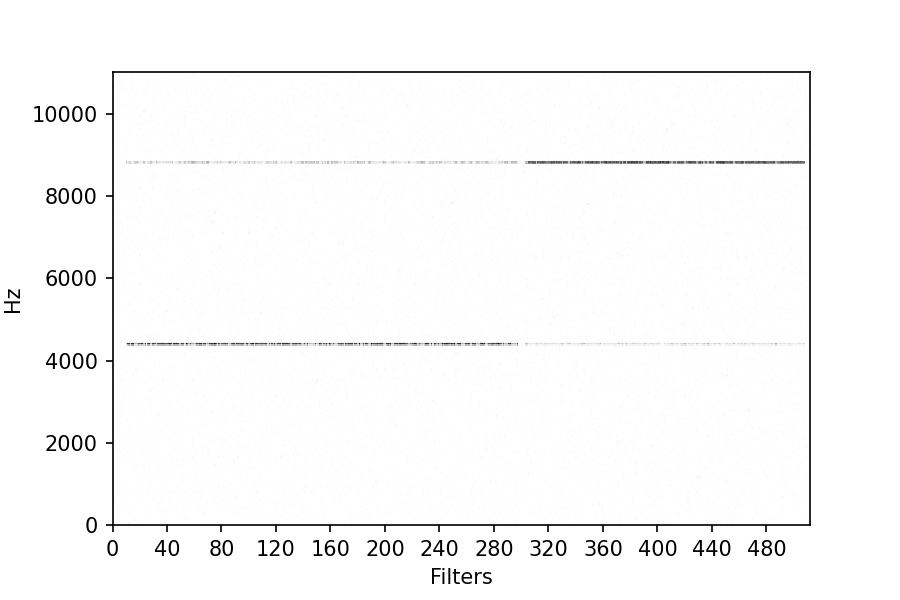
\includegraphics[width=.16\textwidth]{figs/billboard/cpc_spectrum/epoch1490_layer0.png}}\hfill
    \subcaptionbox{CPC$^{(4)}_{\mathrm{Billboard}}$\label{fig:1a}}{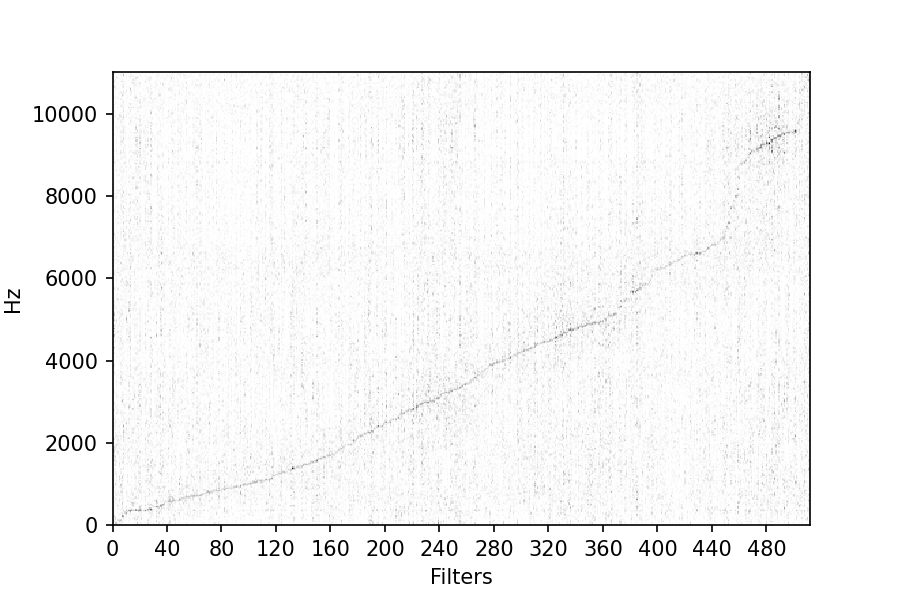
\includegraphics[width=.16\textwidth]{figs/billboard/cpc_spectrum/epoch1490_layer3.png}}\hfill
    \subcaptionbox{CPC$^{(6)}_{\mathrm{Billboard}}$\label{fig:1a}}{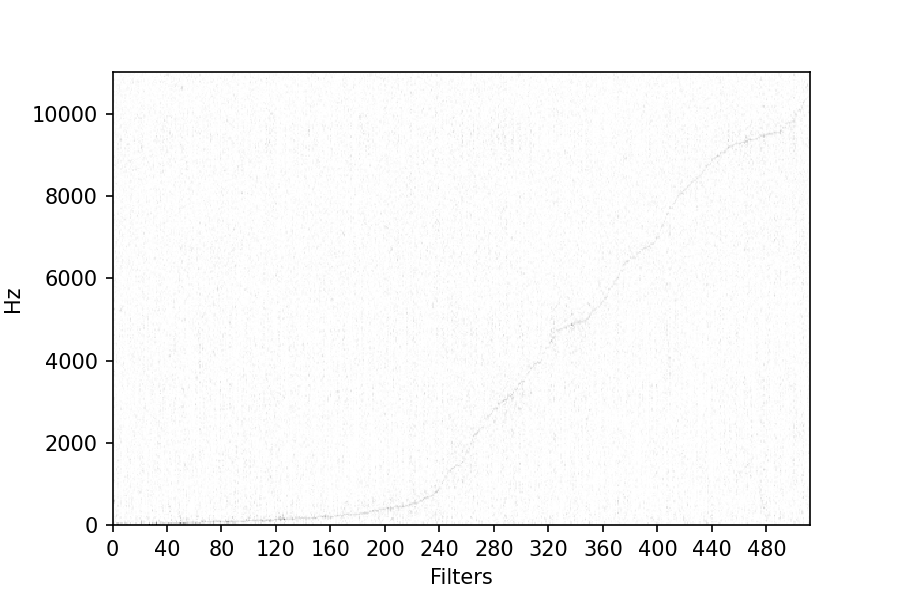
\includegraphics[width=.16\textwidth]{figs/billboard/cpc_spectrum/epoch1490_layer5.png}}

    \caption{Normalised magnitude spectrum of the filters of the self-supervised models in the sample-level convolution layers, sorted by the frequency of the peak magnitude. Gradient ascent is performed on a randomly initialised waveform of 729 samples (close to typical frame size) and its magnitude spectrum is calculated subsequently. Each vertical line in the graph represents the frequency spectrum of a different filter. The first three images are taken from a pre-trained, converged CLMR model, the last three from a CPC model, on the MTAT or Billboard datasets}
    \label{fig:filter_visualisation}
\end{figure*}